\documentclass[report, backcover, french, nodocumentinfo]{upmethodology-document}
\usepackage[utf8]{inputenc}
\usepackage[T1]{fontenc}
%\usepackage{natbib}
\usepackage{csquotes}
%\usepackage[backend=biber,style=alphabetic,citestyle=authoryear]{biblatex}
\usepackage{amsmath}
\usepackage{amssymb}
\usepackage{hyperref}
\usepackage{listings}
\usepackage{textcomp}
\usepackage{color}
\usepackage[toc,page]{appendix}
\usepackage{wrapfig}
\usepackage{stackengine}
\usepackage{scalerel}

%link option, especialy for the table of contents
\hypersetup{
    colorlinks=true,
    linkcolor=black,
    urlcolor=blue,
    linktoc=all
}

\setfrontcover{classic}

\declaredocument{Conception de projet: clone de MiniMetro}{Rapport LO43}{LO43-A2016}
\setpublisher{Université de Technologie de Belfort-Montbéliard}

%\incversion{\makedate{jj}{mm}{aaaa}}{Initial version.}{\upmpublic}
\incversion{\today}{Initial version.}{\upmpublic}

\addauthorvalidator*[julien.barbier@utbm.fr]{Julien}{BARBIER}{Auteur original}
\addauthorvalidator*[maxime.pinard@utbm.fr]{Maxime}{PINARD}{Auteur original}

\addinformed*[franck.gechter@utbm.fr]{Franck}{GECHTER}{Professeur de l'UV LO43}

\setdockeywords{UTBM, LO43, MiniMetro, Java, JavaFX, UML}

\setcopyrighter{Julien BARBIER et Maxime PINARD}
\setpublisher{Julien BARBIER et Maxime PINARD}
\setprintingaddress{France}

%\setfrontcover{modern}
%\setfrontillustration[0.6]{figures/logo}

\graphicspath{./figures/}

%\bibsize{\normalfont}

\newcommand*\cleartoleftpage{%
  \clearpage
  \ifodd\value{page}\hbox{}\newpage\fi
}

\newcommand{\p}[1]{\paragraph{#1\\}}

%Function to print a warning sign
\newcommand{\dangersign}[1][2.5ex]
	{\renewcommand{\stacktype}{L}
		{\scaleto{\stackon[1pt]{\color{red}$\triangle$}{\fontsize{4pt}{4pt}\selectfont !}}{#1}}}

% For more information about UPmethodology: https://www.ctan.org/pkg/upmethodology

\begin{document}

	\upmdocumentsummary{}
	\upmdocumentauthors{}
	\upmdocumentinformedpeople{}
	\upmpublicationpage{}

	\tableofcontents{}
	\listoffigures{}

	\newpage{}
	\chapter{Présentation de Mini Metro}
		\section{Un peu d'histoire...}
			\p{}
				Mini Metro est un jeu développé par le studio indépendant Dinosaur Polo inc. Mini Métro a été présenté sous le nom de Mind The Gap à la 26ème édition du Ludum Dare qui a eu lieu le 26 avril 2013. Il est ensuite développé pour devenir un jeu complet et il est proposés aux Steam Greenlight qui permet au publique de choisir quel jeu indépendant va entrer dans le catalogue Steam de manière permanente ou temporaire. Il sort sous sa forme définitive sur Steam et GOG.com le 6 novembre 2015. Il est ensuite porté sur les plateformes mobiles Android et IOS le 18 octobre 2016.
		\section{But du jeu}
			\p{}
				Mini Metro est un jeu de gestion de métro. On doit gérer les rames de métro pour pouvoir desservir toutes les stations de métro. Ces stations se remplissent, au fur et à mesure du temps, des passagers qui souhaitent aller à une station particulière. En effet, ces stations possèdent une forme et les passagers décident d'aller à une station avec une forme spécifique. Par exemple, un passager arrive à une station triangle et souhaite aller dans une station carré. Il faut donc relier les stations par des lignes et ainsi éviter qu’une station surcharge. Si une station surcharge, la partie se termine.
			\p{}
				Le jeu propose plusieurs niveaux qui se situent chacune dans une ville réelle (New York, Sydney\ldots). Dans chacun des niveaux, on peut rencontrer de nouveaux types de train et le niveau de difficulté change.

		\section{Analyse du jeu}
			\p{}
				Au démarrage du jeu, le joueur a accès à un succinct menu qui nous permet de choisir si on veut jouer, quitter le jeu ou modifier les paramètres de jeu. Si le joueur décide de jouer, il a accès à un autre menu qui lui propose tous les niveaux disponibles et le joueur choisit un niveau. Si celui-ci décide d'entrer dans les paramètres, il aura accès au contrôle de volume et la couleur du fond (blanc ou gris foncés).
			\p{}
				A l'intérieur d'un niveau, le joueur peut tracer des lignes entre les stations. Il possède un inventaire dans lequel il y a de base 3 lignes et 2 trains. Le jeu est en temps réels ainsi tous les éléments du jeu sont fonctions du temps (l'arrivée de station, de passager...). Tous les dimanches, le joueur reçoit des bonus de façon aléatoire avec parfois un choix possibles entre deux bonus.
			\p{}
				Le joueur modifie en temps réel les lignes voir retirer une ligne (il suffit de retirer la lignes de toutes les stations). Si elle est supprimée, la ligne revient dans l'inventaire du joueur. Après modification de la ligne, si un train se situé sur la section de la ligne modifié, celui-ci continue sur l'ancienne section avant la mise à jour. Si une section de la ligne passe dans une partie de l'eau, alors cette section devient un tunnel et on a un nombre limité de tunnel.
			\p{}
				Il peut aussi ajouter ou retirer un train à une ligne. Si le train est retiré, celui-ci retourne dans l'inventaire du joueur. Le joueur peut déplacer un train, mais celui-ci reste immobile pendant 2-3 secondes et les passagers présents avant le déplacement retournent à la station d'origine.

	\chapter{Conception globale du projet}
		\section{Cas d'utilisation}\label{useCases}
			\begin{figure}[h!]
				\centering
				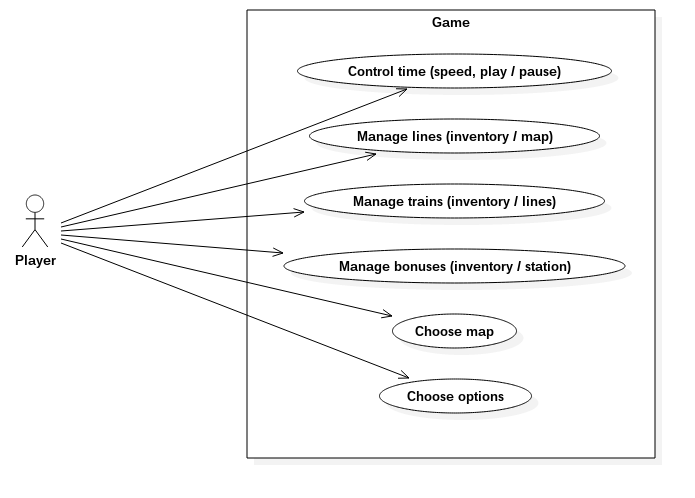
\includegraphics[width=\textwidth]{figures/UseCaseDiagram}
				\caption{Diagramme des cas d'utilisation}
				\label{fig:UseCaseDiagram}
			\end{figure}
			\p{Simulateur}
				MiniMetro a pour particularité d'avoir un fonctionnement proche d'un simulateur, en effet a l'inverse d'un jeu d'échec par exemple qui attend sur l'utilisateur pour effectuer des action, MiniMetro lui a un fonctionnement en temps réel indépendant de l'utilisateur mais dépendant de l’environnement, que l'utilisateur peut modifier. En effet si l'utilisateur ne fait rien, le jeu continue mais cela mènera vite a la défaite, par conséquent l'utilisateur modifie l’environnement (trace des ligne, ajoute de wagons aux trains\ldots) pour empêcher la ``simulation'' d'aller a sa perte.
			\p{Actions de l'utilisateur}
				Les actions de l'utilisateur se répartissent en trois catégories:
				\begin{itemize}
					\item Choix (avant le début de la partie):
						\begin{itemize}
							\item De la carte
							\item Des options de jeu
						\end{itemize}
					\item Ajustement de la vitesse de jeu
					\item Déplacements d'éléments
						\begin{itemize}
							\item De la carte a l'inventaire
							\item De l'inventaire a la carte
							\item D'une position a l'autre (trains)
							\item Même modifier une ligne revient a déplacer les connexion et sous-sections de cette ligne\footnote{La représentation des lignes expliquer ultérieurement}
						\end{itemize}
				\end{itemize}
				Les actions décisives possible une fois en jeux pour l'utilisateur sont donc toutes des déplacements.

		\section{Le modèle MVC}
			\subsection{Adaptation a notre utilisation}
				\p{Choix}
					Nous avons choisit de séparer notre projet en 3 parties: modèle, vue et contrôleur (MCV) pour organiser le code et rendre chaque parie le plus indépendant des autres que possible. Ceci dans le but d'obtenir un code maintenable et facilement adaptable a une autre bibliothèque graphique par exemple puisqu'il suffirait de ré-implémenter une partie de la vue.
				\p{Modèle}
					Il possède toute la logique du jeu il décide a chaque instant de quoi faire et s'adapte en fonction de l’environnement. Environnement qu'il maintient a jour en fonction des modifications dont il est notifier.
				\p{Vue}
					Elle est composée de tout les éléments graphiques du projet et est donc directement dépendante de la bibliothèque graphique utilisé a l'implémentation. Nous utiliserons \textit{JavaFx}.
				\p{Contrôleur}
					Il s'occupe de donner un sens a la vue, transforme les actions abstraites du joueur (glisser sa souris de la position $(14,35)$ a la position $(452,128)$) en action concrète pour le modèle (tracer une ligne de la station $A$ a la station $B$). Il s’occupe aussi le l'action inverse de transformer les action du modèle (déplacer le train) en actions visuelles (déplacer la vue associée au train).
				\p{Prise en compte de JavaFx}
					Puisque notre vue est réalisée par une librairie graphique externe au projet (ici \textit{JavaFx}) nous avons décidé de fusionner le contrôleur et la vue au niveau de la répartition des packages, le package \jpackage{view} regroupant donc les classes de contrôle qui en interne utilisent les éléments de \textit{JavaFx}. On obtient donc deux packages principaux: \jpackage{modele} et \jpackage{view}.
				\p{}
					On arrive donc sur un modèle hybride entre modèle vue (MV) et modèle, vue et contrôleur (MCV) du fait que la séparation contrôleur -- vue qui n'apparait pas au niveau des package, cela étant du a l'utilisation d'une librairie graphique externe au projet. Néanmoins notre conception n'est pas dépendante de \textit{JavaFx} et autre librairie graphique pourrait très bien être utilisée.

	\chapter{Classes et liaisons}
		\subsection{Modèle}
			\p{}
			Pour faire le modèle, nous nous sommes basées sur ce que nous voyons. Ainsi quand on joue, on voit des trains, des lignes et des stations. Une des plus grosse interrogations que nous ayons eu a été les lignes. Pour pouvoir faire des modifications sur la lignes, nous avons décidés de divisée les lignes en sections qui correspond aux rails qui relie deux stations entre elles. Mais cette section peut être composé d'un angle et comme on devaient avoir les coordonnées de cette angle pour la vue, nous avons ainsi des sous-sections au nombre maximum de deux par section. De plus, ces sous-sections permettent de résoudre le problème des tunnels qui peuvent être sur une partie de la section et pas sur l'autre. Ainsi nous obtenons le diagramme UML du Model.
			\begin{figure}[h!]
				\centering
				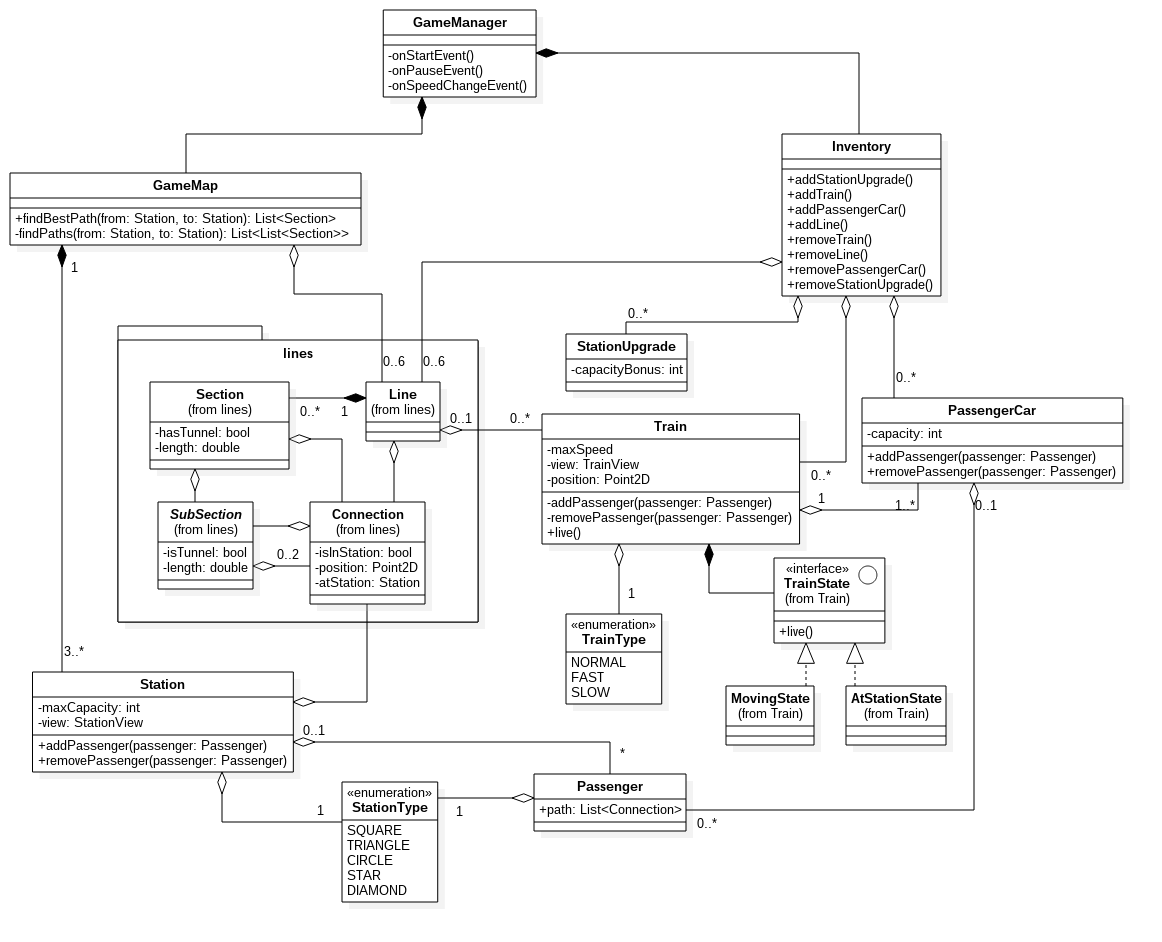
\includegraphics[width=1\textwidth]{figures/ModelClassDiagram} % or <figures/sample.jpg>
				\caption{Diagramme de Classe : Modèle}
				\label{fig:ModelClassDiagram}
			\end{figure}
			\p{}
			Comme on peut le voir sur le digramme \ref{fig:ModelClassDiagram}, nous avons un paquet lines qui contiendra toutes les classe qui décriront les lignes qu'on peut voir dans le jeu. Dans ce packages, les connections correspondent aux point qui séparent les sous-sections au sein de sections. Ces connexions peuvent être au sein d'une stations et permet de résoudre le problème de la connexion d'une station avec plusieurs lignes. En effet, on aura un nombre de connexion dans une station identique au nombre de lignes qui passera dans la station. On pourra ainsi définir une limite de 3 connexions (et donc de trois lignes) au sein d'une station. 
			Une sous-section est composée de 2 connections qui serviront à délimiter la sous-section et ainsi connaitre sa longueur pour pouvoir faire par la suite du path-finding pour les passagers. On retiendra aussi avec le booléen si la sous-section est un tunnel ou pas pour pouvoir décrémenter ou non le compteur de tunnel et compter ceux-ci. On retiendra aussi la longueur de la sous-section. 
			Dans la classe section, on aura le booléen hasTunnel qui permettra de savoir si la section possède un tunnel ou pas, la longueur de la section et les connections d'arrivée et de départ pour délimiter la section. On retiendra aussi  la ligne à laquelle appartient la section.
			Dans la classe Line, on retiendra les connections au sein de celle-ci (pour avoir ainsi les stations qui la constituent). On stocke aussi les trains qui sont présents au sein de la ligne pour le path-finding. On a décidé de faire une composition pour avec les sections. En effet, si on décide de retirer une ligne, on aura plus de section, celle-ci étant détruite.
			\p{}
			Pour les trains, on a la classe Train et PassengerCar où Train est l'objet qui se déplace et le PassengerCar l'objet qui va transporter les passagers. La classe Train est composé de sa vitesse maximum qui va être associé en fonction de l'enum TrainType. En effet, comme dans MiniMetro, on possède plusieurs types de Train en fonction du niveau. Pour pouvoir représenter, nous avons décidé de crée un enum qui aura les différents types de train. Nous avons aussi sa position à un temps donné. Nous avons décidés aussi de faire une state machine pour le problème de la vie du train. En effet, dans la boucle de jeu, le train va appeler la fonction live(). Ainsi, en fonction de s'il est en route ou arrêter en station, le jeu va appeler la fonction live() tout le temps. D'où la state machine qui va permettre au train d'avoir une fonction particulière en fonction de son état. Ainsi la state Machine TrainState va être l'interface qui sera hérité par InMovingState et AtStationState qui implémenteront la fonction live() différemment ce qui permettra d'appeler a fonction live() sans à se soucier de l'endroit où se trouve le train. Le train possède forcément au moins un wagon ou PassengerCar pour pouvoir prendre des passagers aux stations. Donc, le train saura sur quelle ligne il est. Mais le train peut se situer dans l'inventaire et dans ce cas là, le train n'aura pas de ligne.
			\p{}
			La classe Station va contenir les passagers qui veulent aller à une autre station, sa capacité maximum, les connections qu'elles possèdent pour le croisement de lignes et son type qui est ici représenté sous la forme d'un enum appelé StationType.
			\p{}
			C'est différentes classes vont être manipulé par un objet appelé GameManager. Celui-ci va gérer le jeu et possédé la boucle de jeu. La GameMap va contenir tous les objets qui seront présents sur la map (station, lignes, train...). C'est cette objet qui va calculer le path-finding pour chaque passager qui va apparaitre à une station donnée. Celui-ci possédant une référence sur tous les objets présents sur la map, il pourra trouver le chemin optimal pour le passager en question.
		\subsection{Vue}
			La vue n'a pas de encore de conception définitive mais mais sont fonctionnement global a déjà été choisit.
			\subsubsection{Gestion centralisée}
				Notre vue sera gérée par le \jclass{ViewManager}. Ce dernier est celui qui communique avec le modèle (communication détaillé dans les sections suivantes). C'est lui qui instancie les éléments de la vue en fonction de la skin qui lui aura été passé en paramètre de constructeur. Cette skin (dont la conception reste encore a définir) est le groupe d'objets graphiques qui sera utilisé pour représenter les éléments a l'écran, la skin de base étant celle de \textit{MiniMetro} avec des rectangles colorés pour les trains et des formes (triangle, rond, \ldots) pour les stations. Lorsque le \jclass{GameManager} demande une vue pour un train il passe en paramètre le type du train, ainsi le \jclass{ViewManager} crée une vue du type associé avec la skin qui correspond au type du train. Lorsque le train est retiré de la carte, on passe par le \jclass{ViewManager} pour retirer la vue du train de la carte et mettre a jour le compteur de train de l'inventaire. C'est donc le \jclass{ViewManager} qui instancie et gère tout les éléments de la vue.
			\subsubsection{Gestion déléguée}
				Une fois la référence sur la vue fournie au train ou a la station par le biais de l'interface, sa gestion est délégué au train ou station qu'elle représente. Les fonctions de l'interface permettant par exemple pour une station d'ajouter des passagers en précisant juste le type de station vers laquelle ce dernier veut aller et l'implémentation de la vue se charge de prendre le skin associé pour ajouter graphiquement un passager.
			\subsubsection{Contrôle utilisateur}
				Le jeu se joue entièrement a la souris et les interactions de l'utilisateur et comme expliqué dans les cas d'utilisation (voir \ref{useCases}) une fois en jeux il y plusieurs types d'interaction: le contrôle du temps a l'aide de boutons, le choix des bonus lorsqu'il apparaissent et le déplacement d'éléments du jeux.
				\p{Contrôle du temps}
					L'interface graphique contiendra un slider pour régler la vitesse du jeu, un bouton lecture et un bouton pause. A la modification de la vitesse de jeu ou la mise en pause / reprise le \jclass{ViewManager} envoie un event et le \jclass{GameManager} réagit en conséquence pour modifier le temps.
				\p{Choix des bonus}
					Pour le choix d'un bonus le \jclass{GameManager} appel une fonction du \jclass{ViewManager}. Le jeux est en pause le temps que le joueur choisisse un bonus, la fonction peut donc être bloquante. Au cas ou nous aurions besoin de continuer a exécuter des actions dans le thread du \jclass{GameManager}, nous réaliserons une fonction non bloquante qui retourne un \jclass{Futur}.
				\p{Déplacement d'éléments}
					Pour le déplacement des éléments nous avons décidé d'utiliser des états a la façon d'une state machine visibles sur la figure \ref{fig:ModificationStatesClassDiagram}. Le \jclass{ViewManager} aura une référence sur un \jclass{ModificationState}, au clic de la souris en fonction de l'objet pointé on l'assignera au l'état qui correspond (\jclass{MovingTrainState} si c'était un train\ldots) que l'objet soit sur la carte ou dans l'inventaire. On appel aussi la \jfunc{init} pour initialiser l'état (faire apparaitre le train sous la souris\ldots) et instancier les objets graphiques temporaire qui vont permettre une visualisation de la modification par l'utilisateur. Puis tout le long du drag n drop la fonction \jfunc{update} sera appelée pour actualiser ces objets temporaires en fonction (déplacer le train, tracer la ligne jusqu’à la souris\ldots). Au relâchement de la souris la fonction \jfunc{apply} est appelée pour que les objets temporaires soit supprimés, qu'un event soit envoyé et l'action validée par la logique qui modifiera la vue en conséquence (ajouter un train a une ligne\ldots).
					\begin{figure}[h!]
						\centering
						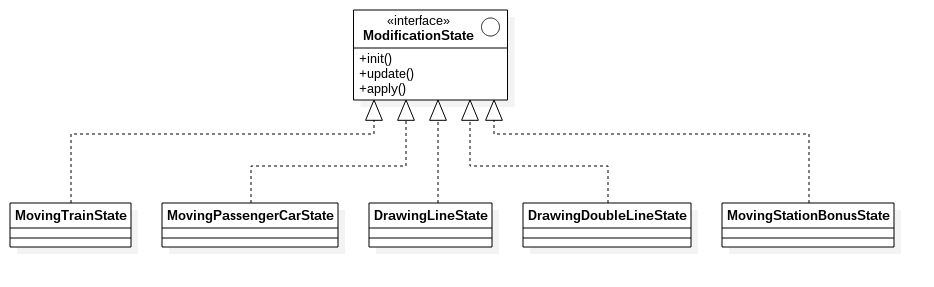
\includegraphics[width=\textwidth]{figures/ModificationStatesClassDiagram.png}
						\caption{Diagramme de classes: Modification states}
						\label{fig:ModificationStatesClassDiagram}
					\end{figure}
					TODO: Explication state en fonction de la souris
		\subsection{Liaison modèle -- vue}
			\begin{figure}[h!]
				\centering
				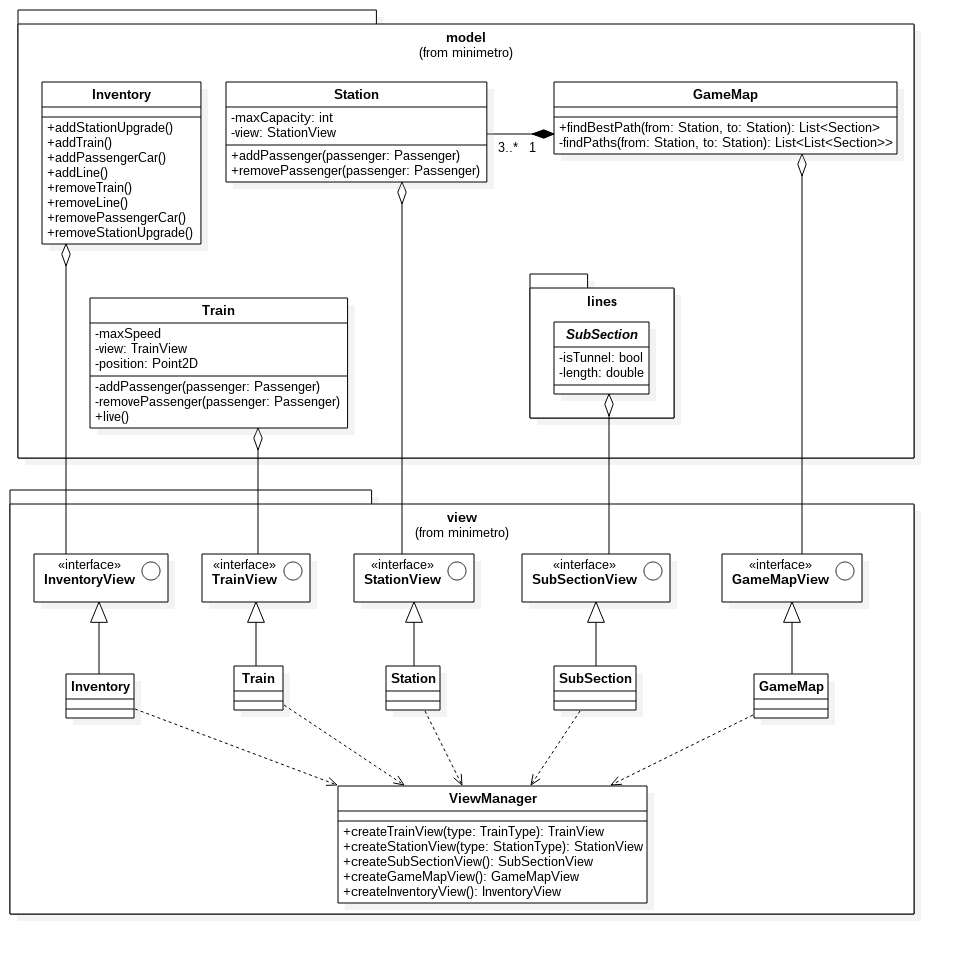
\includegraphics[width=\textwidth]{figures/ModelViewLinkClassDiagram}
				\caption{Diagramme de classes: Liaison modèle -- vue}
				\label{fig:ModelViewLinkClassDiagram}
			\end{figure}
			\p{Choix}
				Nous avons décidés pour pouvoir faire la communication entre le modèle vers la view de faire une communication par interface. En effet, cette solution permet aux modèles d'intérragir de manière immédiat avec la vue et de lui demander une mise à jour de la view de manière simple et légère.
			\p{Fonctionnement}
				Comme on peux le voir avec le diagramme UML \ref{fig:ModelViewLinkClassDiagram}, on a les différentes classes du modèle qui possèdent une interface qui correspond à la vue de celle-ci (par exemple le train possède une \jinterface{TrainView} etc...). Les classes de la vue elle vont implémenter leurs interfaces qui les correspondent(la classe \jclass{Train} du paquet \jpackage{View} va implémenter l'interface \jinterface{TrainView}). Ainsi on a une communication particulière entre les classes du model et de la view. Ainsi si le train veut prévenir la view qu'il existe, il suffira que le train par l’intermédiaire de l'interface signale à la classe \jclass{Train} du paquet \jpackage{View} qu'il existe en appelant une fonction de celle-ci.
		\subsection{Liaison vue -- modèle}
			\subsubsection{Communication par event}
				\p{Choix}
					Nous avons décider que la communication entre la vue et le modèle se ferait par event de façon a ce que la vue n'ait pas de référence sur les éléments du modèle. De cette façon on évite les problème de référencement circulaire qui en Java peuvent empêcher le \texttt{grabage collector} de libérer la mémoire. De plus cela accentue la séparation entre la vue et le modèle.
				\p{Fonctionnement}
					Le principe des events est que certains objets sont des \jclass{EventListener} (implémentent l'interface en Java), c'est a dire qu'il possède une fonction a appeler pour les notifier d'un event, cette fonction est souvent nommée \jfunc{onEvent} et elle contient les actions a effectuer lors de la réception d'un event. Tout ceci utilise des template sur les types des \jclass{Event} qui sont des extensions d'une base class \jclass{Event}. En java on utilisera les \texttt{Generics}.
			\subsubsection{EventDispatcher}
				\p{}
					Nous avons décidé d'utiliser d'utiliser un \texttt{EventDispatcher} pour l'envoi de nos events afin d'éviter le stockage de liste d'\jclass{EventListener} dans toutes nos classes qui envoient des events. Ce dernier a déjà été codé avant le projet, voir figure \ref{fig:EventDispatcherClassDiagram}. Il utilise des \jclass{WeakReference} et n'est donc pas a prendre en compte dans la gestion de la mémoire. De plus il est thread safe.
					\begin{figure}[h!]
						\centering
						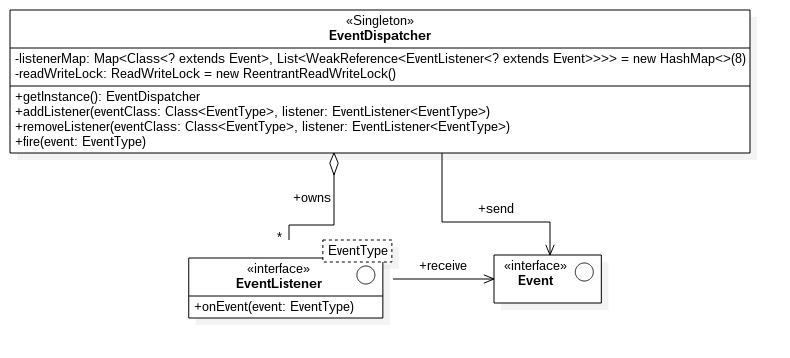
\includegraphics[width=\textwidth]{figures/EventDispatcherClassDiagram}
						\caption{Diagramme de classes: EventDispatcher}
						\label{fig:EventDispatcherClassDiagram}
					\end{figure}
				\p{Fonctionnement}
					L'\jclass{EventDispatcher} est un singleton, il peut être utilisé de n'importe ou avec \jfunc{getInstance}. Les méthodes \jfunc{addListener} et \jfunc{removeListener} permettent de s'enregistrer ou dé-enregistrer en tant que \jclass{EventListener} pour un certain type d'\jclass{Event} passé en paramètre. Pour cela il faut implémenter l'interface \jinterface{EventListener}. Depuis \textit{Java 8} il est aussi possible de passer en paramètre une fonction lambda.
			\subsubsection{Utilisation concrète}
				\p{}
					La figure \ref{fig:ViewModelLinkClassDiagram} représente la liaison entre la vue et le modèle avec les event qui notifient des modification sur la vitesse et mise en pause du jeux a titre d'exemple. Différent types d'events seront crée pour chaque action de l'utilisateur mais la conception de la vue n'étant pas encore définitive et dépendante de \textit{JavaFx} nous n'avons pas encore décidé d'une représentation des données a envoyer dans les events (ex: description de la nouvelle position d'une ligne qui a été modifié).
					\begin{figure}[h!]
						\centering
						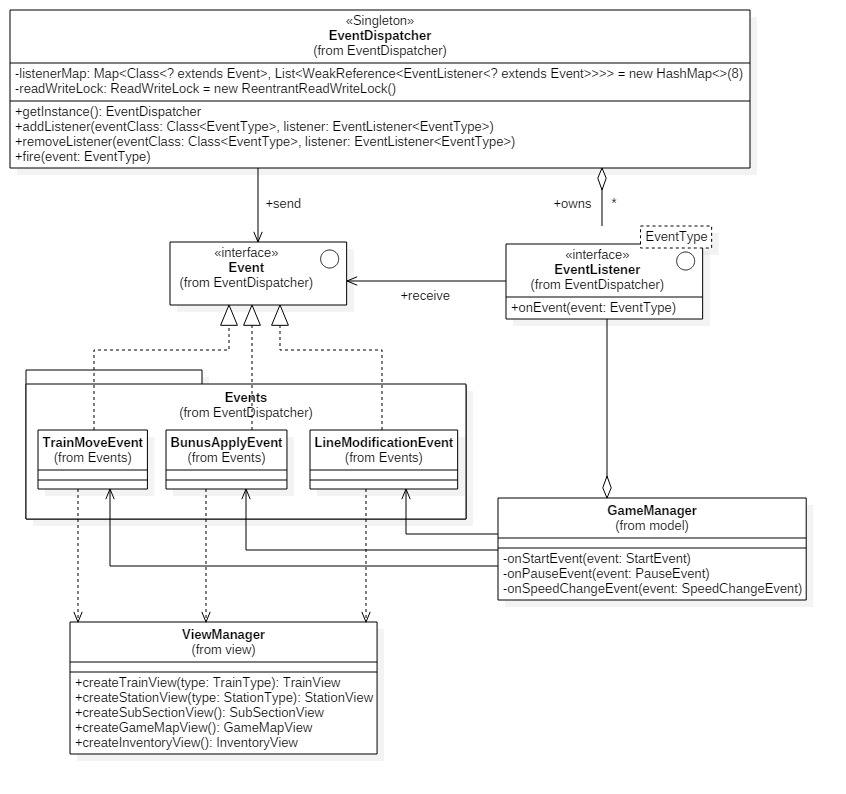
\includegraphics[width=\textwidth]{figures/ViewModelLinkClassDiagram}
						\caption{Diagramme de classes: Liaison vue -- modèle}
						\label{fig:ViewModelLinkClassDiagram}
					\end{figure}
				\p{}
					Concrètement et comme visible sur la figure \ref{fig:ViewModelLinkClassDiagram}, le \jclass{GameManager} possèdes des \jclass{EventListener} qui correspondent a chaque type d'event envoyé par le \jclass{ViewManager}, ces \jclass{EventListener} feront appel aux méthodes \jfunc{onEventXXX} du \jclass{GameManager}. La réceptions des events dans le modèle se fait donc par le \jclass{GameManager} qui modifie le contexte en conséquence. Du coté de la vue, sa conception n'étant pas encore définitive et dépendante de \textit{JavaFx}, il se pourrait que les events ne soient pas tous envoyé par le \jclass{ViewManager} mais qu'il soient envoyé par les éléments directement concerné (par exemple le \jclass{TrainView} pour notifier de son déplacement).

	\chapter{Solutions particulières}
		\section{Gestion du temps}
			TODO: TimeManager\ldots
		\section{Temps réel}
			TODO: Moteur de gestion des trains\ldots
		\section{Description des cartes}
			\p{problème}
				Les cartes de MiniMetro sont plus qu'une simple description de zone puisqu'elles sont entièrement scriptées, les bonus qui apparètrons, le moment ou ils apparetrons, les apparitions de stations, leur forme, position\ldots Sont identiques a chaque partie sur la carte.
			\p{Scripts}
				\begin{figure}[h!]
					\centering
					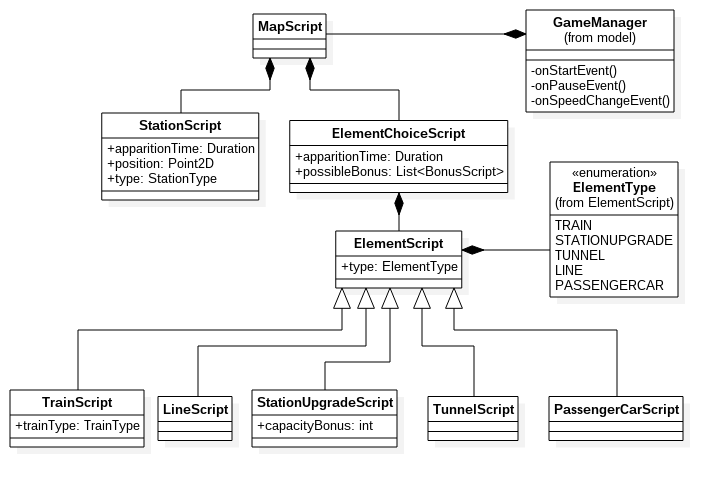
\includegraphics[width=\textwidth]{figures/ScriptsClassDiagram}
					\caption{Diagramme de classes: Scripts}
					\label{fig:ScriptsClassDiagram}
				\end{figure}
				Notre solution, visible sur la figure \ref{fig:ScriptsClassDiagram} a été de crée des classes de description que nous avons nommées scripts. A début d'une partie est créé le \jclass{GameManager}, on passe a ce dernier en paramètre de constructeur un \jclass{MapScript} qui contient toute les informations nécessaire au déroulement de la partie.
			\p{Utilisation}
				La boucle de gameplay principale qui gère principalement les trains s'occupera a chaque tour de boucle de regarder si le timecode du prochain évènement a été dépassé, si c'est le cas il agira en fonction de l'évènement.
			\p{Apparition d'une station}
				Dans le cas ou le timecode d'apparition de la prochaine station a été atteint, le \jclass{GameManager} instanciera une nouvelle \jclass{Station} avec les informations du \jclass{StationScript} tel que la position. Il utilisera la fonction \jfunc{createStationView} du \jclass{ViewManager} en passant en paramètre le type de la station pour obtenir une vue avec le skin associé au type de la station, le \jclass{StationView} retourné sera passé a la \jclass{Station}.
			\p{Choix d'un bonus}
				Les bonus dans Minimétro étant toujours des éléments a ajouté a l'inventaire (train, ligne\ldots), choisir un bonus revient juste a choisir un élément a ajouter a son inventaire. Dans le cas ou le timecode de la sélection du / des prochain bonus est dépassé, le \jclass{GameManager} utilisera les fonction (que nous n'avons pas encore définies) du \jclass{ViewManager} pour demander a l'utilisateur de choisir entre les différent bonus décrit dans le \jclass{ElementChoiceScript}. En fonction du choix de l'utilisateur le \jclass{GameManager} sélectionnera les scripts correspondants et suivra la même procédure que pour les \jclass{Station}. Il instanciera les éléments en fonction du script, leur associera une vue et les ajoutera a l'inventaire. L'énumération \jclass{ElementType} permet de sécuriser les cast.
	\chapter{Notes}
		\section{Modèle MVC}
			\begin{itemize}
				\item model = package model
				\item controlleur = package view
				\item vue = JavaFx, package view
			\end{itemize}
			Liaison vue $\rightarrow$ model:
			\begin{itemize}
				\item Events
				\item Utilisation d'un event dispatcher
			\end{itemize}
			Liaison model $\rightarrow$ vue:
			\begin{itemize}
				\item Interfaces
				\item La réalisation des interface que nous feront sera en JavaFx
				\item Appel au \textit{ViewManager} pour obtenir l'instanciation des vues
				\item ex: la logique demande un train de type \textit{FAST}, le viewManager instancie un \textit{ConcreteTrainView} avec le skin associé a \textit{FAST} et retourne l'interface \textit{TrainView} sur le \textit{ConcreteTrainView}
			\end{itemize}
		\section{Modèle}
			\begin{itemize}
				\item Station
				\item Ligne
					\begin{itemize}
						\item Section
							\begin{itemize}
								\item SubSection
								\item Connection
							\end{itemize}
					\end{itemize}
			\end{itemize}
			Division de manière a pouvoir parcourir une ligne facilement avec un train en suivant les \textit{SubSection} et \textit{Connection} mais aussi éditer au niveau des lignes par les \textit{Section} en fonction de la vue.
		\section{Vue}
			Est en réalité plutôt un contrôleur dans le sens ou JavaFx sera la vue dans notre implémentation.
			\begin{itemize}
				\item A une mini logique interne pour lier les stations par des sections
				\item ViewManager:
					\begin{itemize}
						\item Instancie des réalisations des interfaces de contrôle de la vue
						\item Écoute les events de JavaFx pour en fonction des actions de l'utilisateur prévenir par events le modèle des modifications de l'utilisateur
					\end{itemize}
				\item Éléments de la vue:
					\begin{itemize}
						\item Possède une skin qui est leur apparence graphique
						\item Fonction de gestion de cette vue
					\end{itemize}
			\end{itemize}
		\section{Temps réel}
			\subsection{Contraintes}
			On remarque:
			\begin{itemize}
				\item \textbf{Contrainte 1:} A carte fixe:
					\begin{itemize}
						\item Les éléments qui ont rapport au temp sont les trains
						\item Les autres éléments dépendent des trains (passager qui montent et descendent des stations)
					\end{itemize}
				\item \textbf{Contrainte 2:} Mais la carte est dynamique:
					\begin{itemize}
						\item Apparition des stations
						\item Apparition (dans l'inventaire après choix) des bonus
					\end{itemize}
				\item \textbf{Contrainte 3:} Plus l'utilisateur qui modifie en temp réel la carte
			\end{itemize}
			\subsection{Nos solutions}
				\subsubsection{Contrainte 1}
					\begin{itemize}
						\item Moteur du jeu: boucle de gestion des train
						\item Appelé $X$ fois par secondes: dépendant de la vitesse du jeu qui est réglable
						\item Appel la fonction \textit{live()} de tout les trains en circulation
							\begin{itemize}
								\item Le train est une state machine simplifiée, 2 états: en mouvement et a une station
								\item Le train appel \textit{live()} de son état
									\begin{itemize}
										\item En mouvement: avance en fonction de son accélération / vitesse / direction (dépend de la ligne)
										\item A une station: prend / dépose des passager a une certaine vitesse
									\end{itemize}
								\item A la ``fin'' d'un état (arrive a une station / a déposer et pris tout les passagers nécessaires) le train passe a l'état suivant
							\end{itemize}
						\item Un train enlevé d'une ligne est enlevé de la boucle de jeu et ajouté a l'inventaire
					\end{itemize}
				\subsubsection{Contrainte 2}
					\begin{itemize}
						\item Lorsque l'utilisateur choisit la carte de jeu, un nouvelle partie commence. Pour cela on instancie un \textit{GamaManager} qui prend en paramètre un \textit{MapScript}
						\item Le \textit{MapScript} décrit la carte (position des l'eau), mais aussi le propriétés associés au thème (quel skin utiliser pour les trains\ldots)
						\item Le \textit{MapScript} décrit aussi les événements qui vont arriver au cour de la partie
						\item A	chaque tout de la boucle de jeu on regarde dans le script si un évènement est a réalisé
						\item Deux évènements peuvent avoir lieu:
							\begin{itemize}
								\item Apparition d'une station elle même décrite par un \textit{StationScript} (position, forme\ldots)
								\item Choix d'un ou plusieurs bonus c'est a dire choix d'un élément a ajouter a son inventaire
									\begin{itemize}
										\item \textit{ElementChoiceScript} $\longrightarrow$ \textit{ElementScript} $\longrightarrow$ \textit{TrainScript}, \textit{LineScript}\ldots a expliquer
									\end{itemize}
							\end{itemize}
					\end{itemize}
				\subsubsection{Contrainte 3}
					Les actions qui ne modifient pas la carte (modification de la vitesse de jeu, play, pause, choix de bonus\ldots) déclenchent l'envoi d'event a la logique.\\
					pour les autres:
					\begin{itemize}
						\item Ce sont des déplacements
							\begin{itemize}
								\item De l'inventaire a la carte
								\item De la carte a l'inventaire
								\item A une position invalide $\rightarrow$ retour a la position précédente
							\end{itemize}
						\item Utilisation de state machine simplifiée
						\item Lorsque l'utilisateur clique en fonction de la position de curseur on choisit sélectionne l'état:
							\begin{itemize}
								\item \textit{MovingTrainState}
								\item \textit{DrawingState} (abstract, classes dérivées pour simple ou double ligne)
								\item \ldots
							\end{itemize}
						\item Lorsqu’il bouche la souris on appel \textit{update()} de l'état
						\item Lorsqu'il relâche le clique on appel \textit{apply()} de l'état
							\begin{itemize}
								\item Si le mouvement est valide l'action est effectuée
								\item Sinon l'élément retourne a sa position précédente
							\end{itemize}
					\end{itemize}
		\section{Notes}
			\begin{itemize}
				\item Listes $\Longrightarrow$ shémas
				\item Schéma de fonctionnement du menu? (genre de pushdown automaton)
			\end{itemize}
	%\theupmdockeywords
	%\makebackcover
\end{document}
